%%%%%%%%%%%%%%%%%%%%%%%%%%%%%%%%%%%%%%%%%
% Programming/Coding Assignment
% LaTeX Template
%
% This template has been downloaded from:
% http://www.latextemplates.com
%
% Original author:
% Ted Pavlic (http://www.tedpavlic.com)
%
% Note:
% The \lipsum[#] commands throughout this template generate dummy text
% to fill the template out. These commands should all be removed when 
% writing assignment content.
%
% This template uses a Perl script as an example snippet of code, most other
% languages are also usable. Configure them in the "CODE INCLUSION 
% CONFIGURATION" section.
%
%%%%%%%%%%%%%%%%%%%%%%%%%%%%%%%%%%%%%%%%%

%----------------------------------------------------------------------------------------
%	PACKAGES AND OTHER DOCUMENT CONFIGURATIONS
%----------------------------------------------------------------------------------------

%\documentclass{article}
\documentclass[11pt]{article}
\usepackage{fancyhdr} % Required for custom headers
\usepackage{lastpage} % Required to determine the last page for the footer
\usepackage{extramarks} % Required for headers and footers
\usepackage[usenames,dvipsnames]{color} % Required for custom colors
\usepackage{graphicx} % Required to insert images
\usepackage{subcaption}
\usepackage{listings} % Required for insertion of code
\usepackage{courier} % Required for the courier font
\usepackage{amsmath}
\usepackage{framed}

% Margins
\topmargin=-0.45in
\evensidemargin=0in
\oddsidemargin=0in
\textwidth=6.5in
\textheight=9.0in
\headsep=0.25in

\linespread{1.1} % Line spacing

% Set up the header and footer
\pagestyle{fancy}
\lhead{\hmwkAuthorName} % Top left header
\chead{\hmwkClass\ (\hmwkClassTime): \hmwkTitle} % Top center head
%\rhead{\firstxmark} % Top right header
\lfoot{\lastxmark} % Bottom left footer
\cfoot{} % Bottom center footer
\rfoot{Page\ \thepage\ of\ \protect\pageref{LastPage}} % Bottom right footer
\renewcommand\headrulewidth{0.4pt} % Size of the header rule
\renewcommand\footrulewidth{0.4pt} % Size of the footer rule

\setlength\parindent{0pt} % Removes all indentation from paragraphs

%----------------------------------------------------------------------------------------
%	CODE INCLUSION CONFIGURATION
%----------------------------------------------------------------------------------------

\definecolor{mygreen}{rgb}{0,0.6,0}
\definecolor{mygray}{rgb}{0.5,0.5,0.5}
\definecolor{mymauve}{rgb}{0.58,0,0.82}

\lstset{ %
  backgroundcolor=\color{white},   % choose the background color
  basicstyle=\footnotesize,        % size of fonts used for the code
  breaklines=true,                 % automatic line breaking only at whitespace
  captionpos=b,                    % sets the caption-position to bottom
  commentstyle=\color{mygreen},    % comment style
  escapeinside={\%*}{*)},          % if you want to add LaTeX within your code
  keywordstyle=\color{blue},       % keyword style
  stringstyle=\color{mymauve},     % string literal style
}

%----------------------------------------------------------------------------------------
%	DOCUMENT STRUCTURE COMMANDS
%	Skip this unless you know what you're doing
%----------------------------------------------------------------------------------------

% Header and footer for when a page split occurs within a problem environment
\newcommand{\enterProblemHeader}[1]{
%\nobreak\extramarks{#1}{#1 continued on next page\ldots}\nobreak
%\nobreak\extramarks{#1 (continued)}{#1 continued on next page\ldots}\nobreak
}

% Header and footer for when a page split occurs between problem environments
\newcommand{\exitProblemHeader}[1]{
%\nobreak\extramarks{#1 (continued)}{#1 continued on next page\ldots}\nobreak
%\nobreak\extramarks{#1}{}\nobreak
}

\setcounter{secnumdepth}{0} % Removes default section numbers
\newcounter{homeworkProblemCounter} % Creates a counter to keep track of the number of problems
\setcounter{homeworkProblemCounter}{0}

\newcommand{\homeworkProblemName}{}
\newenvironment{homeworkProblem}[1][Problem \arabic{homeworkProblemCounter}]{ % Makes a new environment called homeworkProblem which takes 1 argument (custom name) but the default is "Problem #"
\stepcounter{homeworkProblemCounter} % Increase counter for number of problems
\renewcommand{\homeworkProblemName}{#1} % Assign \homeworkProblemName the name of the problem
\section{\homeworkProblemName} % Make a section in the document with the custom problem count
\enterProblemHeader{\homeworkProblemName} % Header and footer within the environment
}{
\exitProblemHeader{\homeworkProblemName} % Header and footer after the environment
}

\newcommand{\problemAnswer}[1]{ % Defines the problem answer command with the content as the only argument
\noindent\framebox[\columnwidth][c]{\begin{minipage}{0.98\columnwidth}#1\end{minipage}} % Makes the box around the problem answer and puts the content inside
}

\newcommand{\homeworkSectionName}{}
\newenvironment{homeworkSection}[1]{ % New environment for sections within homework problems, takes 1 argument - the name of the section
\renewcommand{\homeworkSectionName}{#1} % Assign \homeworkSectionName to the name of the section from the environment argument
\subsection{\homeworkSectionName} % Make a subsection with the custom name of the subsection
\enterProblemHeader{\homeworkProblemName\ [\homeworkSectionName]} % Header and footer within the environment
}{
\enterProblemHeader{\homeworkProblemName} % Header and footer after the environment
}

%----------------------------------------------------------------------------------------
%	NAME AND CLASS SECTION
%----------------------------------------------------------------------------------------

\newcommand{\hmwkTitle}{Written Homework 1} % Assignment title
\newcommand{\hmwkDueDate}{Thrusday, Jan 24, 2019} % Due date
\newcommand{\hmwkClass}{CSC421} % Course/class
\newcommand{\hmwkClassTime}{LEC 5101} % Class/lecture time
\newcommand{\hmwkAuthorName}{Zhongtian Ouyang} % Your name
\newcommand{\hmwkAuthorID}{1002341012} % Your ID

%----------------------------------------------------------------------------------------
%	TITLE PAGE
%----------------------------------------------------------------------------------------

\title{
\vspace{2in}
\textmd{\textbf{\hmwkClass:\ \hmwkTitle}}\\
\normalsize\vspace{0.1in}\small{Due\ on\ \hmwkDueDate}\\
\vspace{0.1in}
\vspace{3in}
}

\author{\textbf{\hmwkAuthorName}\\ \textbf{\hmwkAuthorID}}

\date{} % Insert date here if you want it to appear below your name

%----------------------------------------------------------------------------------------\
\begin{document}

\maketitle
\clearpage

%----------------------------------------------------------------------------------------
%	Common Tools
%----------------------------------------------------------------------------------------
%\begin{framed}
%\begin{lstlisting}[language=matlab]
%\end{lstlisting}
%\end{framed}

% \begin{bmatrix}
%0.5 & 0.6 \\ 
%0.7 & 0.8
%\end{bmatrix}

%\begin{figure}[h!]
%\centering
%\includegraphics[width=0.6\linewidth]{q10a.png}
%\label{fig:q10a}
%\end{figure}\\

%\begin{figure*}[!ht]
%\begin{subfigure}{.5\textwidth}
% \centering
%  \includegraphics[width=.5\linewidth]{p4_1.JPG}
%  \caption{Full set}
%  \label{fig:sfig1}
%\end{subfigure}
%\begin{subfigure}{.5\textwidth}
% \centering
%  \includegraphics[width=.5\linewidth]{P4_2.JPG}
%  \caption{Two each}
%  \label{fig:sfig2}
%\end{subfigure}%
%\caption{Part4 (a)}
%\label{fig:p4a}
%\end{figure*}

%\sum_{n=1}^{\infty} 2^{-n} = 1
%\prod_{i=a}^{b} f(i)
%----------------------------------------------------------------------------------------
%	PROBLEM 1
%----------------------------------------------------------------------------------------

% To have just one problem per page, simply put a \clearpage after each problem
\begin{homeworkProblem}

\noindent \textit{Hard-Coding a Network}\\
$$ W^{(1)} = 
\begin{bmatrix}
1 & -1 & 0 & 0 \\
0 & 1 & -1 & 0 \\
0 & 0 & 1 & -1 
\end{bmatrix}
, b^{(1)} = 
\begin{bmatrix}
0 \\
0 \\
0 
\end{bmatrix}
, W^{(2)} = 
\begin{bmatrix}
-1 \\
-1 \\
-1 
\end{bmatrix}
, b^{(2)} = 0$$



\end{homeworkProblem}
\clearpage
%----------------------------------------------------------------------------------------
%	PROBLEM 2
%----------------------------------------------------------------------------------------

\begin{homeworkProblem}
\noindent \textit{Backprop}\\

a)
\begin{figure}[h!]
\centering
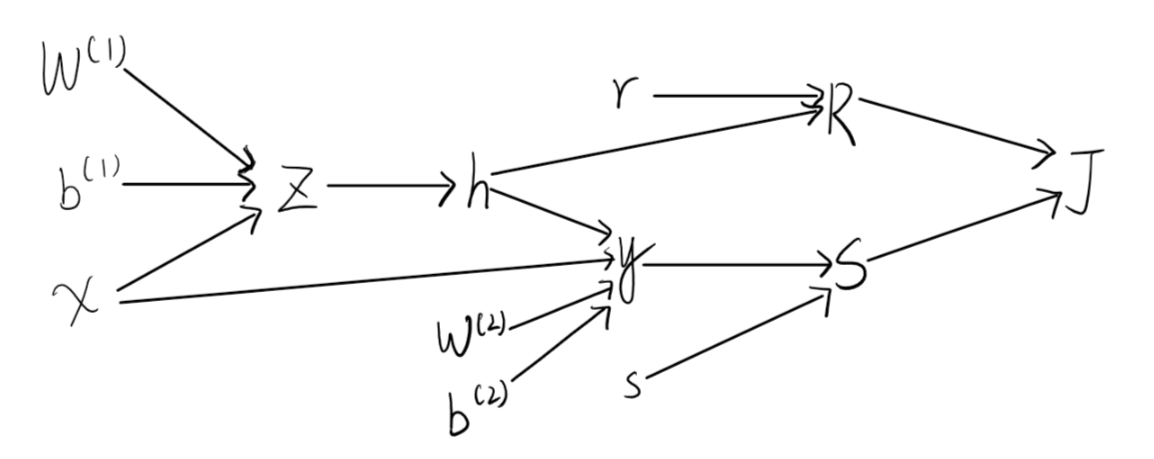
\includegraphics[width=\linewidth]{hw1p1.png}
\label{fig:q2a}
\end{figure}\\
b)\\
$$
\bar{R} = \frac{\partial J}{\partial R}  = 1,
\ \bar{S} = \frac{\partial J}{\partial S}  = 1,
\ \bar{\mathbf{y}} = \bar{S}\frac{\partial S}{\partial \mathbf{y}} = 1*\begin{bmatrix}
\frac{\partial S}{\partial y_1} \\
\vdots \\
\frac{\partial S}{\partial y_n} 
\end{bmatrix}
=
\begin{bmatrix}
y_1-s_1 \\
\vdots \\
y_n - s_n
\end{bmatrix} 
= \mathbf{y - s}
$$
$$
\bar{\mathbf{h}} = \frac{\partial J}{\partial \mathbf{h}}
= \frac{\partial R}{\partial \mathbf{h}} \bar{R} + \frac{\partial \mathbf{y}}{\partial \mathbf{h}}^T \bar{\mathbf{y}}
= 
\begin{bmatrix}
\frac{\partial R}{\partial h_1} \\
\vdots \\
\frac{\partial R}{\partial h_k} 
\end{bmatrix} * 1 + 
\begin{bmatrix}
\frac{\partial y_1}{\partial h_1} & \cdots  & \frac{\partial y_1}{\partial h_k}\\
\vdots & & \vdots\\
\frac{\partial y_n}{\partial h_1} & \cdots  & \frac{\partial y_n}{\partial h_k}
\end{bmatrix}^T \bar{\mathbf{y}}
= 
\begin{bmatrix}
r_1 \\
\vdots \\
r_k
\end{bmatrix}
+
\begin{bmatrix}
w_{11}^{(2)} & \cdots  & w_{1k}^{(2)}\\
\vdots & & \vdots\\
w_{n1}^{(2)} & \cdots  & w_{nk}^{(2)}
\end{bmatrix}^T \bar{\mathbf{y}}
= \mathbf{r} + \mathbf{W}^{(2)T}\bar{\mathbf{y}}
$$
$$
\bar{\mathbf{z}} = \frac{\partial J}{\partial \mathbf{z}} 
= \bar{\mathbf{h}} \frac{\partial \mathbf{h}}{\partial \mathbf{z}}
= \bar{\mathbf{h}}
\begin{bmatrix}
\frac{\partial h_1}{\partial z_1} & \cdots  & \frac{\partial h_1}{\partial z_k}\\
\vdots & & \vdots\\
\frac{\partial h_k}{\partial z_1} & \cdots  & \frac{\partial h_k}{\partial z_k}
\end{bmatrix}
= 
\bar{\mathbf{h}}
\begin{bmatrix}
\sigma^{'}(z_1) &  & 0\\
 & \ddots & \\
0 &   & \sigma^{'}(z_k)
\end{bmatrix}
=\bar{\mathbf{h}} \circ \sigma^{'}(\mathbf{z})
$$
$$
\bar{\mathbf{x}} = \frac{\partial J}{\partial \mathbf{x}} 
= \frac{\partial \mathbf{z}}{\partial \mathbf{x}}^T\bar{\mathbf{z}} + \bar{\mathbf{y}}\frac{\partial \mathbf{y}}{\partial \mathbf{x}}
= \mathbf{W}^{(1)T}\bar{\mathbf{z}} + \bar{\mathbf{y}}
\begin{bmatrix}
\frac{\partial y_1}{\partial x_1} & \cdots  & \frac{\partial y_1}{\partial x_n}\\
\vdots & & \vdots\\
\frac{\partial y_n}{\partial x_1} & \cdots  & \frac{\partial y_n}{\partial x_n}
\end{bmatrix}
=\mathbf{W}^{(1)T}\bar{\mathbf{z}} + \bar{\mathbf{y}}
\begin{bmatrix}
1 &  & 0\\
 & \ddots & \\
0 &   & 1
\end{bmatrix}
= \mathbf{W}^{(1)T}\bar{\mathbf{z}} + \bar{\mathbf{y}}
$$
$$
\bar{x_i} = (\sum_{j=1}^{k} W^{(1)}_{ji}\bar{z_j}) + \bar{y_i}
$$
\clearpage

\end{homeworkProblem}
%----------------------------------------------------------------------------------------
%	PROBLEM 3
%----------------------------------------------------------------------------------------

\begin{homeworkProblem}
\noindent \textit{Sparsifying Activation Functions}\\

$\frac{\partial L}{\partial w_1}$: YES\\
$$\frac{\partial L}{\partial w_1} = \frac{\partial L}{\partial y}\frac{\partial y}{\partial w_1} = \frac{\partial L}{\partial y}\times h_1 = \frac{\partial L}{\partial y} \times 0 = 0$$

$\frac{\partial L}{\partial w_2}$: YES\\
$h_1 = ReLU(z_1)$ where $z_1$ is the input of $h_1$ and $z_1 = -1$. $\partial h_1/ \partial z_1 = ReLU'(z_1) = ReLU'(-1) = 0$
$$\frac{\partial L}{\partial w_2} = \frac{\partial L}{\partial h_1} \frac{\partial h_1}{\partial z_1} \frac{\partial z_1}{\partial w_2} = \frac{\partial L}{\partial h_1} \times 0 \times h_3 = 0$$

$\frac{\partial L}{\partial w_3}$: No\\
$$\frac{\partial L}{\partial w_3} = \frac{\partial L}{\partial h_3} \frac{\partial h_3}{\partial z_3} \frac{\partial z_3}{\partial w_3}$$
$h_3 = ReLU(z_3)$ where $z_3$ is the input of $h_3$ and $z_3$ can be greater than zero, so $\partial h_3/ \partial z_3 = ReLU'(z_3)$ could be 1. $\partial z_3 /\partial w_3 = x_1$ could also be non-zero.
$$\frac{\partial L}{\partial h_3} =\frac{\partial L}{\partial y}\frac{\partial y}{\partial h_3} 
= \frac{\partial L}{\partial y}(\frac{\partial y}{\partial h_1}\frac{\partial h_1}{\partial z_1}\frac{\partial z_1}{\partial h_3} + \frac{\partial y}{\partial h_2}\frac{\partial h_2}{\partial z_2}\frac{\partial z_2}{\partial h_3})
=\frac{\partial L}{\partial y} (w_1\times ReLU'(z_1)\times w_2 + w_5 \times ReLU'(z_2)\times w_4)$$
As stated in the question, $z_1 = -1, ReLU'(z_1) = 0$. However, $z_2$ could be above zero. In that case, $ReLU'(z_2) = 1$
$$\frac{\partial L}{\partial h_3} 
= \frac{\partial L}{\partial y} (w_1\times 0 \times w_2 + w_5 \times 1 \times w_4)
= \frac{\partial L}{\partial y} \times w_5 \times w_4$$
Since $\partial L/ \partial h_3, \partial h_3/ \partial z_3, \partial z_3/ \partial w_3$ can all be non-zero, $\partial L/ \partial w_3$ is not guaranteed to be zero.\\

\end{homeworkProblem}
%----------------------------------------------------------------------------------------
\end{document}
